\documentstyle[pubref,times,twocolumn,epsfig,ieee-iros2000]{article}
\pubref{Proceedings of the IEEE/RSJ International Conference on Intelligent 
        Robots and Systems (IROS 2001)}
       {pages 1226-1231, Wailea, Hawaii, 29 October - 3 November, 2001.}


\newcommand{\xsection}[1]{
  \vspace*{-2em}
  \section{#1}
  \vspace*{-1em}
}
\newcommand{\xsubsection}[1]{
  %\vspace*{-1em}
  \subsection{#1}
  \vspace*{-1em}
}
%\usepackage{graphicx}
%\graphicspath{{.}{./graphics/}{/home/vaughan/tex/graphics/}}

%\usepackage{ieee-iros2000}
%\usepackage{epsfig}
%\usepackage{subfigure}

%\usepackage{vmargin}
%\setmarg{17mm}{4mm}{180mm}{239mm}

\date{}
\title{Most Valuable Player: A Robot Device Server for
  Distributed Control}

\author{Brian P.~Gerkey  \and
  Richard T.~Vaughan \and Kasper St{\o}y \and Andrew Howard \and
  Gaurav S.~Sukhatme \and Maja J~Matari\'{c} \and \\
  Robotics Research Labs, University of Southern California\\
  Los Angeles, CA 90089-0721, USA}

%%\numberofauthors{3}
%%\author{
%%\alignauthor 
%%Brian P.~Gerkey \and
%%Richard T.~Vaughan  \and
%%Kasper St{\o}y  \and
%%Andrew Howard  \and
%%Gaurav S.~Sukhatme \and
%%Maja J~~Matari\'{c} \and  \\ \\
  %%\affaddr{Robotics Research Labs, University of Southern California}\\
  %%\affaddr{Los Angeles, CA 90089 USA}\\
  %%\texttt{\{gerkey|vaughan|ahoward\}@robotics.usc.edu}
%%}

\begin{document}
\maketitle
\pagestyle{empty}
\thispagestyle{empty}

\begin{Abstract}
\vspace*{-1em}
Successful distributed sensing and control require data to
flow effectively between sensors, processors and actuators on single
robots, in groups and across the Internet. We propose a mechanism for
achieving this flow that we have found to be powerful and easy to use; we
call it {\sl Player}.  Player combines an efficient message protocol
with a simple device model.  It is implemented as a multi-threaded TCP
socket server that provides transparent network access to a collection
of sensors and actuators, often comprising a robot.  The socket
abstraction enables platform- and language-independent control of these
devices, allowing the system designer to use the best tool for the
task at hand.  Player is freely available from
\verb+http://robotics.usc.edu/player+.
\end{Abstract}



\xsection{Introduction}
\label{intro}

\begin{figure*}
\begin{center} 
 %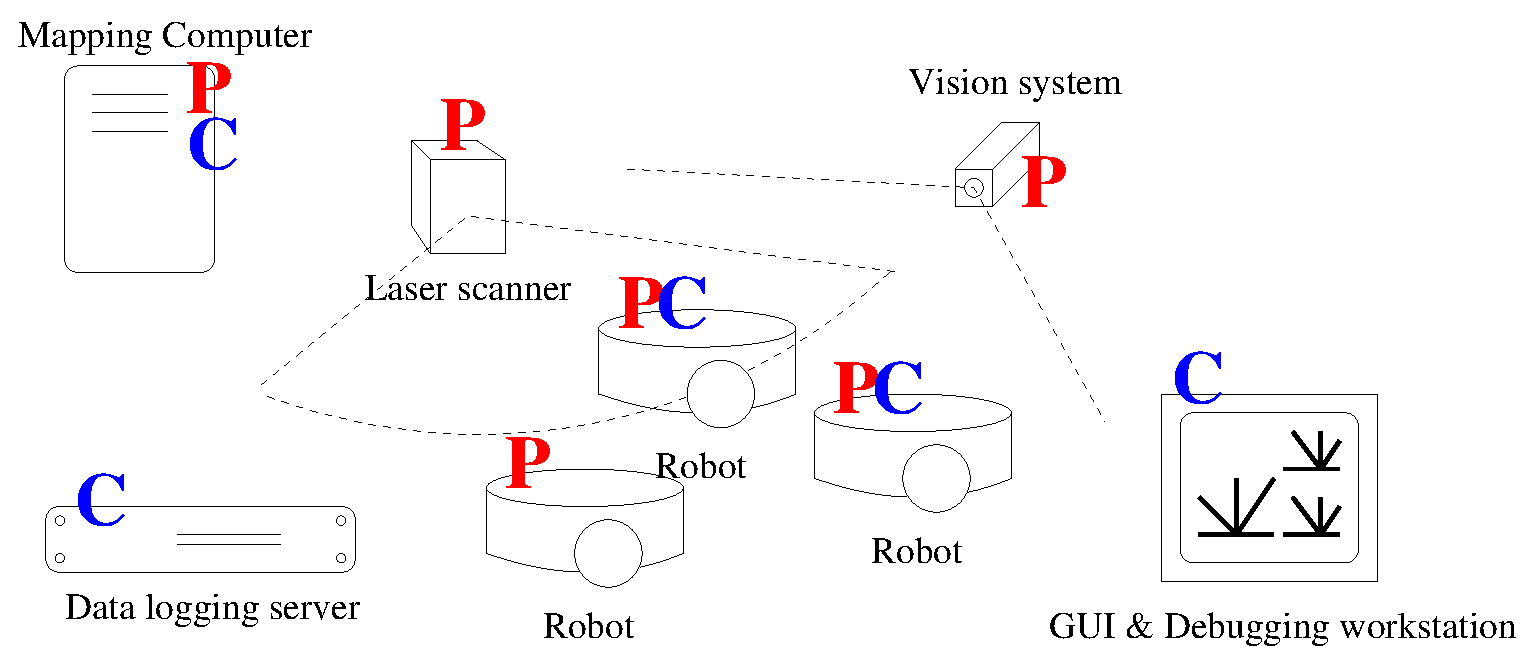
\includegraphics[width=.95\textwidth]{scenario}
 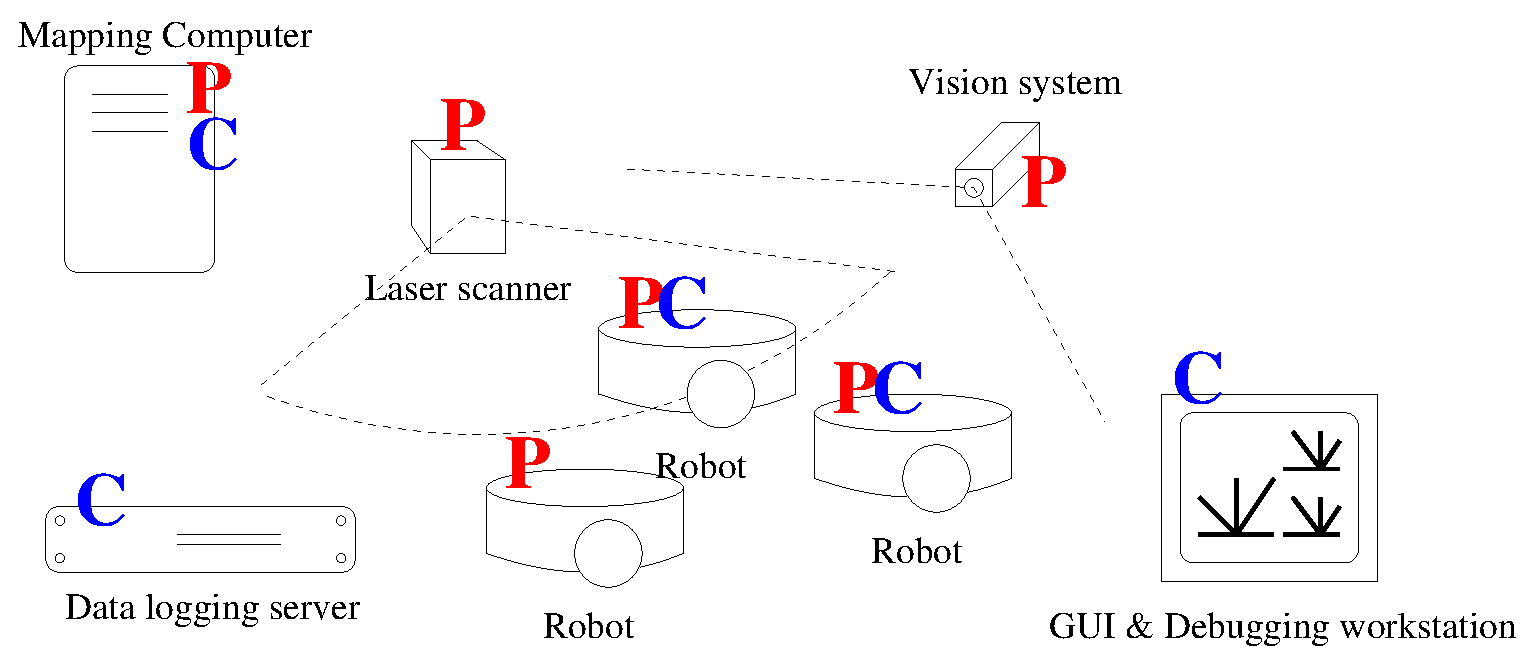
\epsfig{file=scenario.eps, width=.7\textwidth}
 \caption{{\sl Example scenario: Player servers (indicated with a `P') 
     distribute sensor data to clients (indicated with a `C')
     across a network of wired and wireless connections.
     \label{fig:scenario}}}
\end{center}
\end{figure*}

Since 1999, the robots at the University of Southern California
Robotics Research Labs have had on-board TCP/IP and 802.11 wireless
Ethernet as standard equipment. The same is true of many labs around
the world; today the cost, availability and ease of use of the
equipment has put it within reach of most professional and academic users.
Communication with and between robots in the lab is now cheap and
easy. Better still, it supports the standard socket interface; the
system that moves sensor data between processes on the robot's
on-board computer will just as easily move them to the workstation
across the lab or to the web page across the Internet.

We are using this equipment to provide transparent network access to
all sensing and control of our robots. This paper describes our
software {\em Player}, a network server interface to a collection of
sensors and actuators, typically constituting a robot. Player has
quickly become the most-used interface to the hardware in our lab.

There are three main motivations for providing a socket-based robot
server:

%\begin{enumerate}
  
%\item 
{\bf Distribution:} A client has access to sensors and actuators
  anywhere on the network. Clients can connect to multiple servers;
  servers accept connections from multiple clients. A single program
  could control the behavior of several robots; several programs could
  control different aspects of one robot's behavior.  Section
  \ref{scenario} describes a scenario which illustrates some
  possibilities of remote sensing and control.
  
%\item 
{\bf Independence:} Clients can be written in any language and
  on any hardware platform that implements sockets; most languages support
  this today. The user can choose the most appropriate language and
  environment for the task at hand; be it C for run-time speed, Java
  for ease of use, MatLab for algorithm prototyping, Perl for web
  integration, or Tcl/Tk for GUI design.

%\item 
{\bf Convenience:} The server provides an abstract unified
  interface to the devices attached to it. Client programs (robot
  controllers, sensor data processors, etc.) `subscribe' to a set of
  devices and specify the frequency at which data should arrive.  Data
  from the subscribed devices come as one data packet at the
  requested interval. Distribution adds to this convenience, for
  example enabling remote display and logging of robot state and
  sensor data. Some of the earliest Player clients were
  visualization tools for debugging.

%\end{enumerate}

While distribution provides the primary scientific benefit by enabling
an interesting and little-explored class of algorithms, the
independence and convenience are of practical interest to researchers
and students.  Player's ease of use make it attractive even with a
single client running on-board a single robot. Player also interfaces
with {\it Stage} (Section \ref{stage}) to simulate a population of
devices interacting in a virtual environment.

Player is primarily a protocol, as specified in the manual
\cite{GerkeyStoyVaughan00}. 
Any program implementing the protocol counts as a Player. Currently there
is a single implementation; our Player program written in C++ using
POSIX services. It has been tested on Linux and Solaris and should
compile on any POSIX-compliant system. 

Player was written to support our labs' research. Some similar system
is a prerequisite for any exploration of distributed sensing, control
and coordination. The Player experiment has been so successful
in-house that we believe it will be of immediate use to the robotics
and sensor network communities.


\xsection{Scenario}
\label{scenario}
To illustrate how Player can be used to support distributed sensing
and control in a variety of ways, we consider the following scenario,
also shown in Figure \ref{fig:scenario}: An experimental team of
robots patrols a building at Western University, holding a tight
formation. A formation-control program runs on one of the robots. It
subscribes to the sonar range sensors and wheel motors on all three
robots, sending wheel speed commands to maintain a fixed range and
bearing between them. On another robot, a client subscribes to the
audio devices of its host and its closest team-mate, processing the
two audio streams to find the direction of interesting sounds.

Meanwhile an experimenter is debugging the formation controller; she
examines the robots' sonar readings from a GUI client running on her
workstation. A logging server keeps a record of the robots'
ground-truth positions for the experimenter's future paper. The logger
subscribes to the tracking device running on an overhead vision
system.

Simultaneously, a colleague at Eastern University with access to a
supercomputer runs an on-line mapping client that subscribes to every
available ranging device at Western U., including a wall-mounted laser
scanner and the three robots' sonars. The mapping application is not
controlling any actuators, so the 300ms transmission delay over the
Internet is not a problem. However, the map generated is available
online in case a Western robot should need it.

This scenario, while complicated, is fully supported by the current
Player protocol and implementation. Further, we already have examples of
many of these clients.
\begin{figure*}
 \centering
 %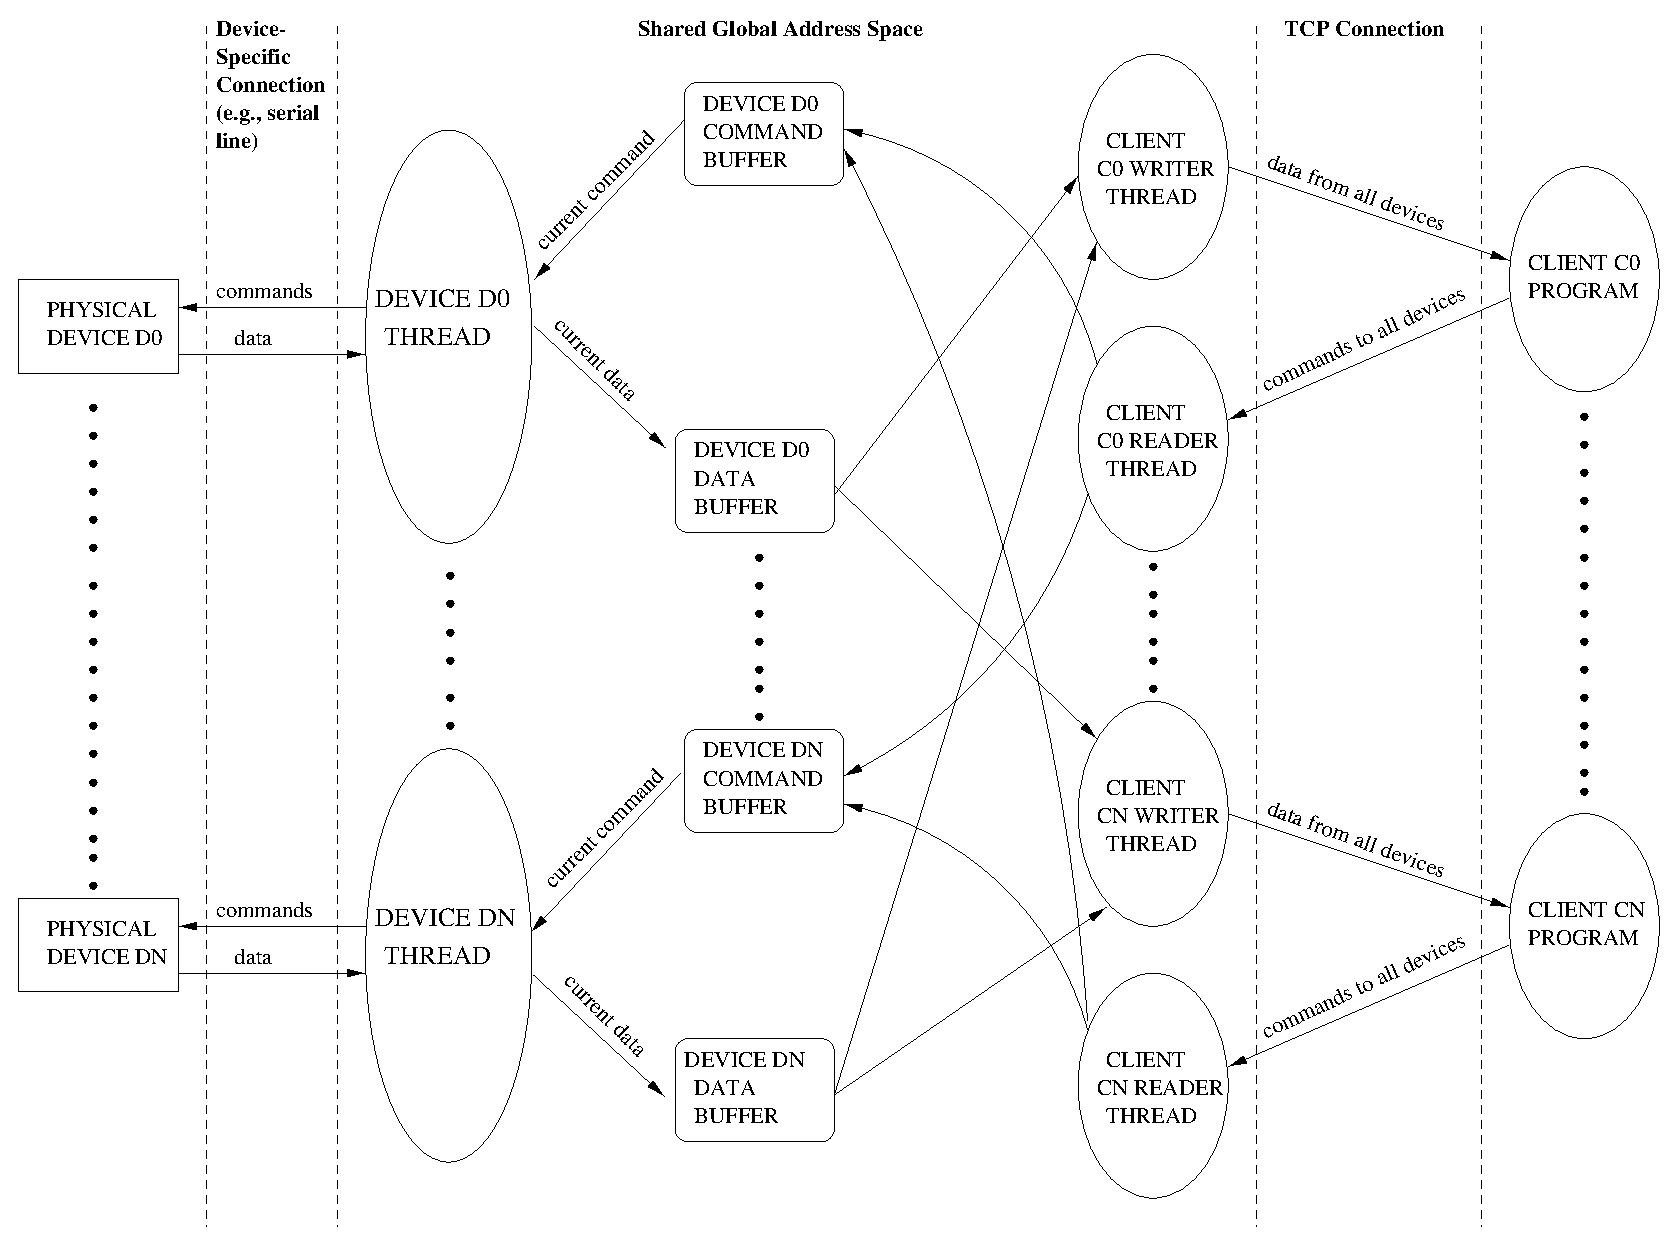
\epsfig{file=buffers.eps, width=120mm, height=75mm}
 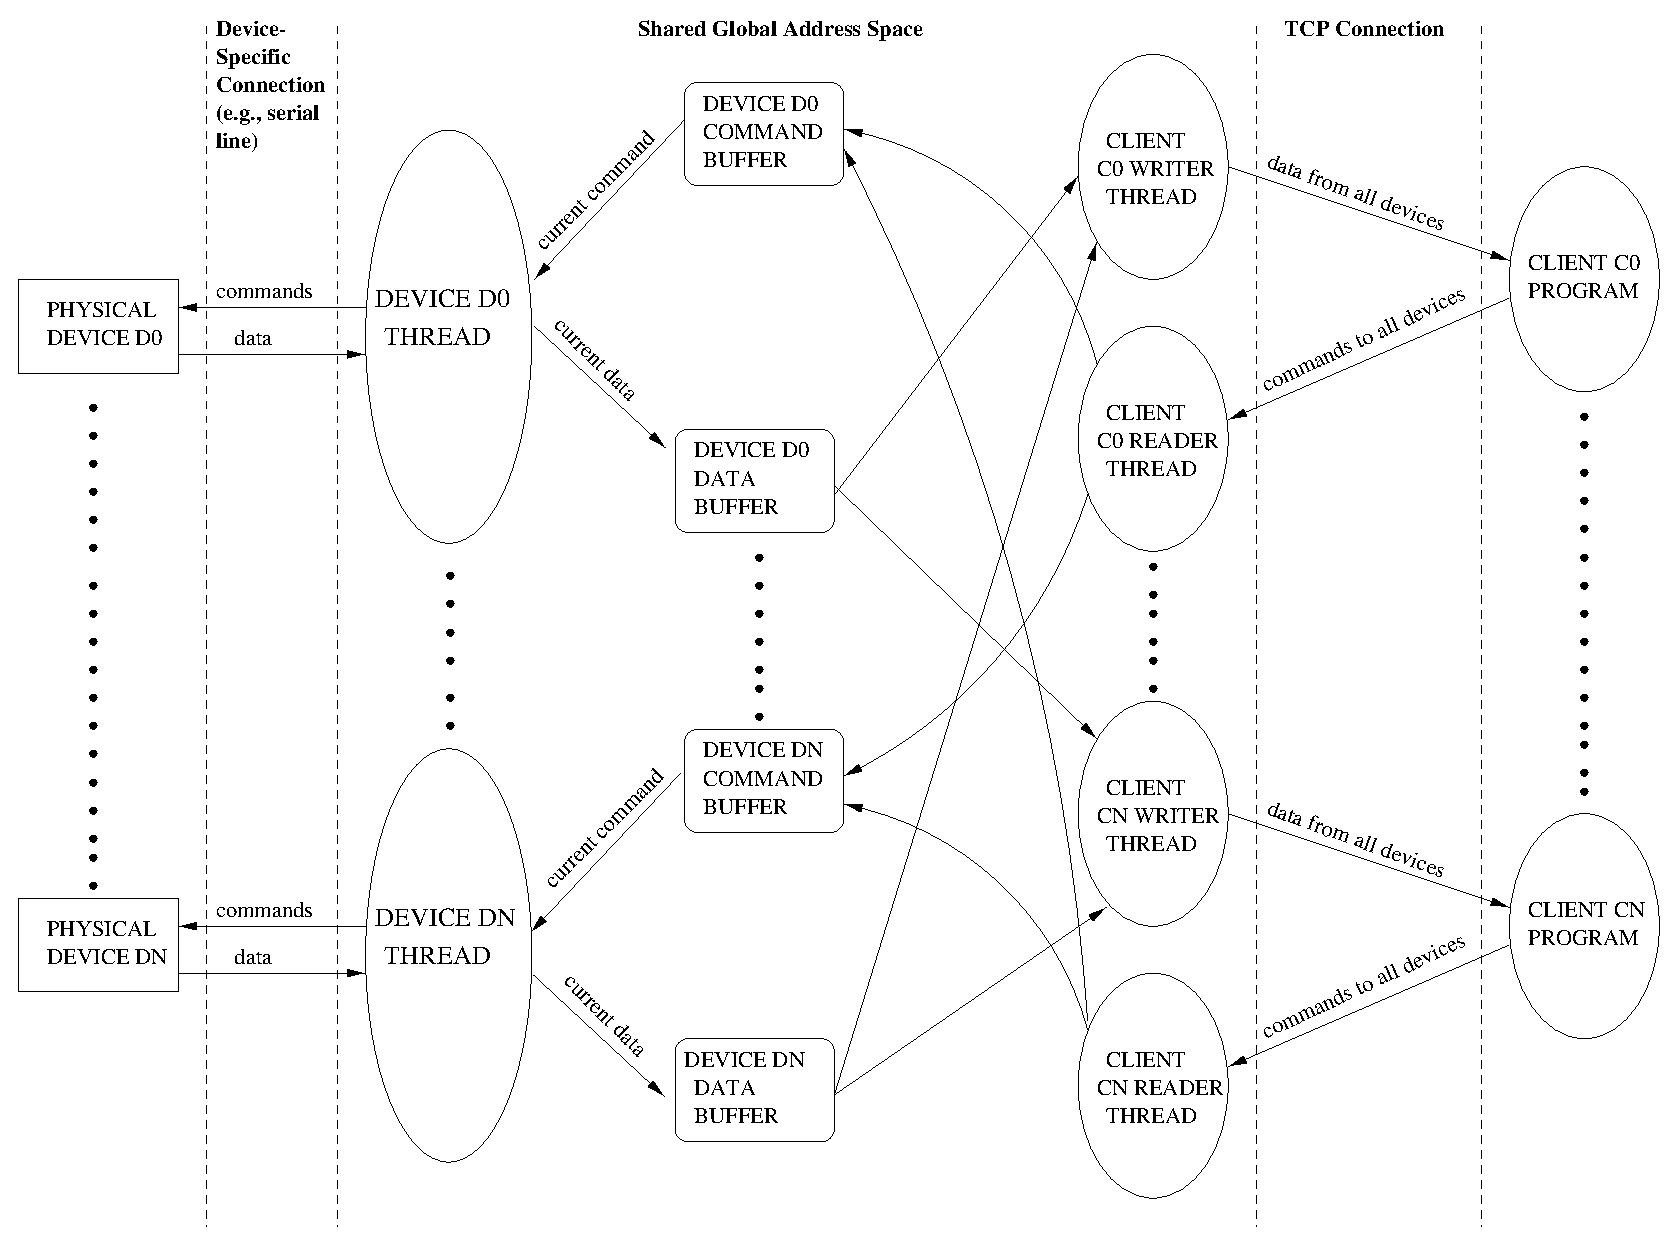
\epsfig{file=buffers.eps, width=.7\textwidth}
  \caption{{\sl Overall system architecture of Player}}
  \label{figure:buffers}
\end{figure*} 

\xsection{Related Work}
\label{related}
Previous work in the area of robot programming interfaces has focused
primarily on providing a development environment that suits a
particular control philosophy.  For example, Ayllu \cite{Werger00},
which, like Player, can be used to control the ActivMedia Pioneer robots,
provides tools for creating concurrent behaviors and, further,
enforces a behavior-based control structure \cite{Arkin98}.  Similarly,
COLBERT/Saphira \cite{Konolige97}, which can also control the Pioneer
robots (among others), is concerned mainly with the construction of
fuzzily-blended behavior-based control systems
\cite{SaffiottiRuspiniKonolige93}.  While such tools are very useful,
we believe that implementing them at such a low level imposes
unnecessary restrictions on the programmer, who should have the choice
to build any kind of control system while still enjoying device
abstraction and encapsulation. Thus in Player
we make a clear distinction between the {\sl programming interface} and 
the {\sl control structure}, opting for a maximally
general programming interface, with the belief that users will develop
their own tools for building control systems.  Further, most
robot interfaces confine the programmer to a single language:
Ayllu uses something akin to C, Saphira uses something akin
to LISP, and TeamBots \cite{balch98} uses Java.  
In contrast, the TCP socket abstraction of Player allows for the 
use of virtually any programming language.
%Finally, both Ayllu and Saphira are commercial
%software products and, as such, cannot be modified by the researcher
%(e.g., to fix bugs, add new devices), nor can the source code be
%studied for educational purposes.  So we wrote our own robot interface
%which will always be Free Software.

The system that is most similar to (and certainly some inspiration
for) Player is the {\scshape Trip} server \cite{Jennings98}; the main
difference between the two is that whereas {\scshape Trip} was
designed as a sophisticated server to support extremely simple
clients, we strove for minimalism in our server and simplicity in our
message protocol, at the possible expense of causing the client to do
more work.

Many other distributed device control and event service systems have
been developed, but we are not aware of one that provides the tradeoff
between power and simplicity that makes Player well-suited to
multi-agent robotic device control.

% TODO: add other stuff, maybe CORBA (GISC-based something something)

\xsection{Architecture}
\label{architecture}

Player's development was guided 
by our desire to concurrently support many heterogeneous devices and many
heterogeneous clients.  Each device operates at some inherent frequency, 
with wide variation among devices.
For example, the popular SICK LMS 200 laser range-finder 
returns a full scan at approximately
5Hz, while the Sony EVID30 pan-tilt-zoom camera can give encoder feedback 
at almost 2500Hz. 
Similarly, each client operates at some inherent frequency;
while a simple client written in C++ may be capable of consuming new data 
at 100Hz, a graphically intensive client written in Tk might operate
at less than 1Hz.  
We want to move data and commands between clients and devices
at the highest rate possible in order to fully exploit the hardware 
and maximize the responsiveness of the system.  

\xsubsection{Server Structure}
Given the requirement to support interaction with external entities
(i.e., clients and physical devices) that operate at different
timescales, we designed Player in the standard model of an
asynchronous threaded server.
Player is implemented in C++ and makes extensive use of the POSIX-compliant
{\tt pthread} interface. 
A main thread listens for new client connections on a well-known TCP
port, spawning threads on demand to service clients and the devices
they request.
%This is less expensive that it may seem; 
%these threads all use blocking I/O and so spend almost their entire
%lives blocked, either on a client, a device, or a timer (see 
%Section~\ref{section:results} for performance figures).
The overall system structure of Player is shown in
Figure~\ref{figure:buffers}.  The center portion of the figure
is Player itself; on the left are the physical devices and
on the right are the clients.  Each client has
a TCP socket connection to Player. If the client is executing on the
same host as Player, then this socket is simply a loopback connection;
otherwise, there is a physical network in between the two.  At the other end,
Player connects to each device by whatever method is appropriate for
that device (e.g., RS-232).

Within Player the threads communicate through a shared global
address space.  As indicated in Figure~\ref{figure:buffers}, each
device has associated with it a command buffer and a data buffer.
These buffers
provide an asynchronous communication channel between the device
threads and the client reader and writer threads.  For example, when
a client reader thread receives a new command for a device,
it writes the command into the command buffer for that device.
Later, when the device thread is ready for a new
command, it will read the command from its command buffer and send
it on to the device.  Similarly, when a device thread receives
new data from its device, it writes the data into its data
buffer.  Later, when a client writer thread is ready to send new
data from that device, it reads the data from the data
buffer and passes it on to its client.  In this way, the client
service threads are decoupled from the device service threads (and
thus the clients are decoupled from the devices).  Also, by the
nature of threads, the devices are decoupled from each other,
and the clients are decoupled from each other.

\xsubsection{Device Model}
In order to provide a uniform abstraction for a variety of devices, we
chose to follow the UNIX model of treating devices as files.  Thus the
familiar file semantics hold for Player devices.  For example, to
begin receiving sensor readings, the client opens the appropriate
device with {\tt read} access; likewise, before controlling an
actuator, the client must open the appropriate device with {\tt write}
access\footnote{Devices in Player can also be configured similarly
to {\tt ioctl()}.}.  
As this model has served UNIX-like operating systems well for
many years, we expect that it will suffice for the devices the Player
will control in the future.

Player currently supports a number of devices, including the
popular Pioneer research robot and various peripherals (for a complete
list, see the Player home page, listed in Section~\ref{section:obtain}).
We have also introduced the concept of {\sl virtual} devices.  Rather
than being tied directly to a piece of hardware, a virtual device performs
aggregation and processing on data gathered from one or more other sensors,
and exports the result.  By integrating useful algorithms directly
into Player, we can easily share expertise and reuse code 
throughout the lab (and the world).


\xsubsection{Client Interaction}
By default, clients receive data at 10Hz\footnote{We chose 10Hz 
because most of our currently supported devices operate at or near that 
frequency.}.
Thus, every 100ms, a client can expect to receive a data packet containing
the current data from all the subscribed devices.  
Of course, by sending all the data at once, Player might repeatedly send old 
data from a device that operates at less than 10Hz.  
We designed Player in
this way for one reason: simplicity.  By always transmitting the current
state for all subscribed devices, regardless of the timescale of the
device, we facilitate the writing of client programs.  As a result,
clients are able to use a simple blocking read loop to receive data 
from Player.  If the client is multi-threaded (many are),
the blocking read could be compartmentalized to a single thread, 
allowing the rest of the client program to proceed unhindered.

Of course, receiving data at 10Hz may not be reasonable for all
clients; for these situations, we provide a method for changing the
frequency, and also for placing the server in a request/reply mode.
So, if a client wants vision data at full frame rate, it can configure
Player to send data at 30Hz, with the tradeoff that it will also
receive (sometimes repeated) data from the other currently requested 
devices at the higher
rate.  Alternatively, if there is a low-bandwidth connection between
Player and a client using laser data (which is comparatively large),
that client might lower the data rate to 5Hz in order to minimize
message-passing and thus conserve bandwidth, with the tradeoff that
data from other requested devices will also arrive more 
slowly\footnote{If a client requires different data rates from 
devices, it can simply make separate connections 
to the server, one for each device.}.  It is
important to remember that even when a client receives data slowly,
there is no backlog and it always receives the most current data; it
has simply missed out on some intervening information.  Also, these
frequency changes affect the server's behavior with respect to each
client individually; the client at 30Hz and the client at 5Hz can be
connected simultaneously, and the server will feed each one data at
its preferred rate.

Analogous to the issue of repetition of old data is the fact that there
is no guarantee that a command given by a client will ever be sent to
the physical device.  Player does not implement any device
locking, so when multiple clients are connected to 
a Player server, they can both write into 
a single device's command buffer.  In general, there is no queuing of 
commands, and each new command will overwrite the old one; 
the service thread for the device will only send to the device itself 
whatever command it finds each time it reads its command buffer.  We
chose not to implement locking in order to provide maximal power and
flexibility to the client programs.  In our view, if multiple
clients are concurrently controlling a single device, such as a robot's
wheels, then those clients are probably cooperative, in which case they
should implement their own arbitration mechanism at a higher level than
Player.  If the clients are not cooperative, then the subject of research
is presumably the interaction of competitive agents, in which case device
locking would be a hindrance.



\xsection{Evaluating the implementation}
\label{section:results}
\begin{figure}
\begin{center} 
  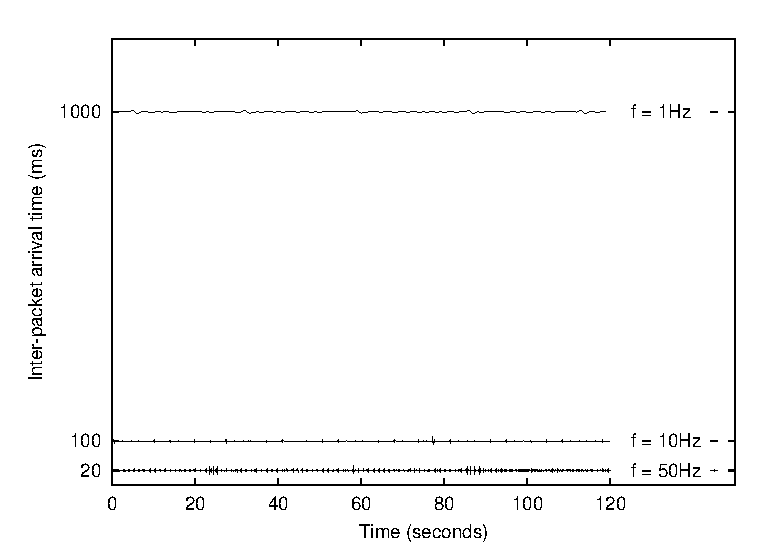
\epsfig{file=1.eps,width=.95\columnwidth}
  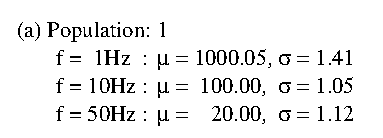
\epsfig{file=cap1.eps,height=10mm}
  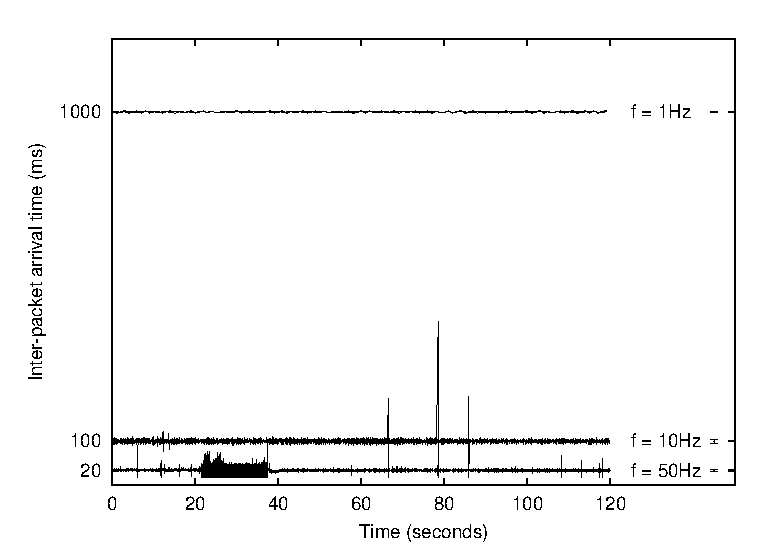
\epsfig{file=10.eps,width=.95\columnwidth}
  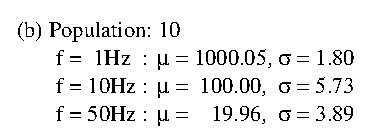
\epsfig{file=cap2.eps,height=10mm}
  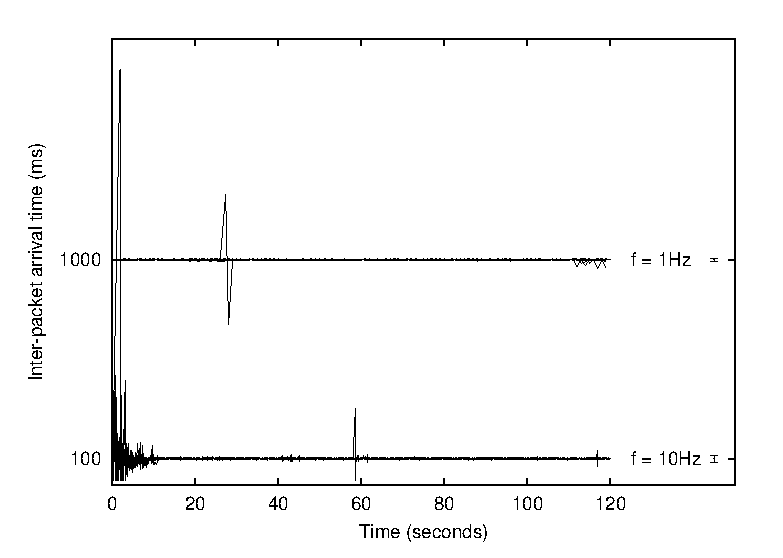
\epsfig{file=50.eps,width=.95\columnwidth}
  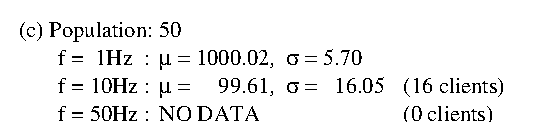
\epsfig{file=cap3.eps,height=10mm}
 \caption{{\sl Inter-packet arrival times measured while serving
          large amounts of sensor data across wireless Ethernet
          to different client populations.}}
  \label{figure:graphs}
\end{center}
\end{figure}
To evaluate the performance of our Player implementation, we performed
a series of stress tests\footnote{These tests were conducted with
Player version 0.8d.}. A number of simultaneous connections were
made to a Player server, and data were requested from a typical set of
devices. We performed 54 experiments, testing all combinations of the
following parameters:

%\begin{itemize}
%\item 
{\bf Number of clients} \{1, 10, 50\}

%\item 
{\bf Client update frequency} \{1, 10, 50Hz\}

%\item 
{\bf Data size} \{small (85 bytes), large (807 bytes)\}

%\item 
{\bf Network type} \{loopback, Ethernet, 802.11\}

%\end{itemize}
\noindent For each of the 54 parameter combinations, we ran the system for 2
minutes and measured the end-to-end data packet latency\footnote{The
  test computers' clocks were synchronized with the network time
  protocol (NTP) \cite{RFC1305}, which can maintain precision of less
  than 1ms.} and time interval between arriving data packets
for each connected client.  End-to-end latency is the sum of network
latency and Player-induced delay due to the asynchronous client and
server loops.  This delay is bounded above by the lesser of the
update intervals of the client and device;  the expected value
of the delay will be half the lesser interval.
A more interesting metric is the
inter-packet arrival time, as it captures Player's ability to maintain
a requested data rate; if a client asks for updates at 10Hz, then, if
Player is working properly, the client will receive a data packet
every 100ms.

In all but the extreme case described below, Player was able to track
the desired data rate very closely. The mean interval between packets
was always $<50{\mu}s$ from the target interval (less than our clock
precision).

Player is therefore generally able to provide data in a timely manner.
However, we observed that in the toughest case we examined,
transferring large packets via 802.11 (of the networks tested, the
wireless has the least bandwidth [at $\approx$1.9Mbps] and 
greatest overhead), Player was
unable to support the larger populations of subscribers. In these
cases some or all of the clients' connections were broken by Player.
Due to lack of space we present here only these {\it worst} performing
results.  Figure~\ref{figure:graphs} plots the measured
time interval between packets received. For a population $P=1$ client,
Player is able to maintain 20, 100 \& 1000ms intervals with little
variance (Figure~\ref{figure:graphs}(a)). For $P=10$ the 1000ms interval is
maintained as before. The 100 and 20ms intervals are also maintained as
means, but increased variance is observed
(Figure~\ref{figure:graphs}(b)). For $P=50$ the 1000ms interval is
maintained, but again with relatively large variance. For the 100ms
interval, Player was found to close connections to 34 of the 50 clients,
leaving only 16 connected which it served at 100ms with high variance.
When 50 clients connected requesting 20ms update rates, Player closed
all connections within a few seconds and no data were served
(Figure~\ref{figure:graphs}(c), no plot for 20ms interval).

These results allow us to determine rough upper bounds for Player's
performance.  For example, the server is unable to handle 50 clients
requesting laser data at 10Hz across the wireless network, but it will
work across the 10Mbps wired Ethernet.  Our initial estimates of the
bandwidth requirements of this service seem to show the wireless is
sufficient. Our next step is to examine these failures more closely to
determine if we are up against a hardware/OS limit, or whether our
implementation can be improved.



\xsection{Stage}
\label{stage}
Stage simulates a population of Player devices, allowing development
and testing of clients in an environment very similar to that provided
by the real hardware. Stage spawns several copies of Player, replacing
the real device drivers with its simulated equivalents. The user
interfaces with Player in the normal way; clients see the identical
interface to real and simulated hardware. 
%As in Player, devices are
%implemented as modules and can be easily added or modified by a
%moderately experienced programmer.

%Stage provides a graphical user interface to the world and its
%devices, allowing the experimenter to easily manipulate devices (e.g.
%moving robots around in the world; panning camera devices, etc.).
%Stage also provides a logging mechanism that is independent of Player
%for ground-truthing.

We have found that agents developed in simulation will work with
little or no modification on the real devices and vice-versa. The
Stage distribution includes a variety of environments suitable for
large and small-scale experiments in multi-agent sensing,
communications and control.

\xsection{Usage}
\label{usage}
Player is the default interface for the Pioneer robots at USC and has
been used for many projects. Incoming graduate students write their
first single-robot controllers for it, and it is used with Stage for
graduate courses in robotic sensing and planning,

Some examples of our research projects using Player (and its precursor
{\it ArenaServer}) are ant-inspired trail-following in robot teams
\cite{VaughanStoySukhatmeMataric00}, cooperative box pushing and multiple target
tracking \cite{GerkeyMataric00}, reducing interference in teams by
aggressive behavior \cite{VaughanStoySukhatmeMataric00a}, investigation of
interaction between network and behavior designs \cite{weiye2000},
simultaneous localization and mapping \cite{HowardMataricSukhatme01}, 
and online resource allocation \cite{OstergaardMataricSukhatme01}.

%\vspace*{1em}
\xsection{Conclusion and future work}
In this paper we have attempted to make explicit some opportunities
presented by ubiquitous network communications for robotics. We have
identified a niche for a novel piece of software that provides
language and platform independent network access and an abstract
interface to collections of sensors and actuators: a {\em Robot device
  server}. Player is our candidate design for such a server.  We have
described it here and made the source and documentation available for
evaluation by the community.

Our Player implementation is deliberately simple and is based on the
well-understood multi-threaded blocking server design. A modular
device driver interface makes adding additional devices straightforward.

We are working on an implementation for the QNX real-time operating
system for use with the USC AVATAR robot helicopter. We also aim to
create a lightweight, low memory, low thread-count version for
handhelds and small embedded devices. The Player protocol and
implementations will evolve as we push them with more complex clients,
additional I/O devices and smaller server platforms.

\label{section:obtain}
Player and Stage distributions, including source code, example 
client programs
and documentation are freely available under the GNU 
General Public License at the
Player home page: \verb+http://robotics.usc.edu/player+.

The acid test of Player will be its uptake. We hope that Player will
develop over the next few years into a well-used tool. It will not
suit every application, but it has proved useful in a variety of roles
in our labs. Our work would be less fun without it.

\renewcommand{\baselinestretch}{0}
{\small
\begin{Acknowledgment}
\vspace*{-1.3em}
This work is supported by 
DARPA contract DAAE07-98-C-L028,
DARPA grant DABT63-99-1-0015,
JPL contract No. 1216961,
NSF grants ANI-9979457 and ANI-0082498 and
ONR grants N00014-00-1-0140, N0014-99-1-0162 and N00014-00-1-0638.

Many thanks to Boyoon Jung, Jakob Fredslund and 
Esben \O{}sterg\aa{}rd for their testing, fixes and ideas.

%The names {\it Player} and {\it Stage} are due to William Shakespeare.
%{\small
%\begin{quote}
  %``All the world's a stage, \\
  %And all the men and women merely players: \\
  %They have their exits and their entrances; \\
  %And one man in his time plays many parts,''\\
  %\hspace*{4em}{\sl As You Like It} Act II, Sc.7
%\end{quote}
%
%\begin{quote}
  %``Life's but a walking shadow, a poor player \\
  %That struts and frets his hour upon the stage \\
  %And then is heard no more: it is a tale \\
  %Told by an idiot, full of sound and fury, \\
  %Signifying nothing.''\\
  %\hspace*{4em}{\sl Macbeth} Act V, Sc.5
%\end{quote}
%}
\end{Acknowledgment}

\bibliographystyle{plain}
\vspace{-2.7em}
\bibliography{robot}
}

\end{document}

